\chapter{Clustering}

\section{Kmeans}
Kmeans is a good general clustering technique. It attempts to group your data into a specified number of clusters. Luckily R has an inbuilt function \verb|kmeans| that can be used.

\begin{center}
	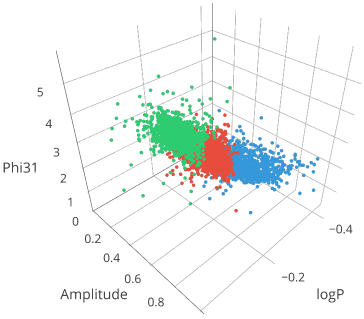
\includegraphics[width=0.5\textwidth]{images/kmeans_01.png}
\end{center}

To use \verb|kmeans| you must first pull out the features of the data that you want to cluster on. Then you can pass the data into the kmeans function, specifying the number of clusters that you want, and it will return information about the generated clusters.

\begin{verbatim}
myData <- offABClustering[,c("logP", "phi31", "amp.I")]
clusters <- kmeans(myData, 3)
\end{verbatim}

If you want to pull out just the cluster ids that kmeans generates in order to store that information in your dataframe, you can pull it out as a \verb|cluster| feature and turn it into a factor.

\begin{verbatim}
offABClustering$cluster <- factor(clusters$cluster)
\end{verbatim}

\section{Support Vector Machines}
Support Vector Machines are a clustering technique that tries to separate data using a linear line, however through the use of kernels it is able transform the data space to give clusters that are non-linear in normal space.

\begin{center}
	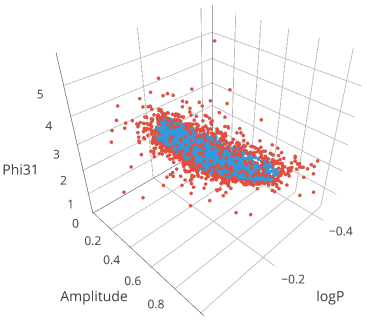
\includegraphics[width=0.5\textwidth]{images/ksvm_01.png}
\end{center}

There are several libraries in R for using support vector machines (SVM).

\begin{itemize}
	\item \verb|kernlab|
	\item \verb|e1071|
\end{itemize}

Let's take a look at the \verb|kernlab| library for now. To cluster data using an SVM with kernlab you need to pull out just the features you want and then convert that dataframe into a matrix. Then you can pass the resulting matrix into the ksvm function.

\begin{verbatim}
myData <- offABClustering[,c("logP", "phi31", "amp.I")]
myMatrix <- as.matrix(myData)
ksvmModel <- ksvm(myMatrix)
\end{verbatim}

The ksvm function will give you a model which you can then use to classify your data into the calculated clusters.

\begin{verbatim}
predictions <- predict(ksvmModel, myData)
offABClustering$cluster <- as.factor(predictions)
\end{verbatim}

\subsection{Kernels}
The ksvm function offers a few different kernels that you can use to change how it clusters the data. Each of these kernels will cluster the data into different shapes ranging from linear separations to rings. It looks like ksvm uses the \verb|rbfdot| kernel by default.

\begin{itemize}
	\item \verb|rbfdot| Radial Basis kernel "Gaussian"
	\item \verb|polydot| Polynomial kernel
	\item \verb|vanilladot| Linear kernel
	\item \verb|tanhdot| Hyperbolic tangent kernel
	\item \verb|laplacedot| Laplacian kernel
	\item \verb|besseldot| Bessel kernel
	\item \verb|anovadot| ANOVA RBF kernel
	\item \verb|splinedot| Spline kernel
\end{itemize}

You can specify the kernel to be used in ksvm, by adding a kernel parameter where you pass in the name of the kernel you want to use as a string.

\begin{verbatim}
ksvmModel <- ksvm(myMatrix, kernel = "vanilladot")
\end{verbatim}

\begin{longtable}{ c c }
	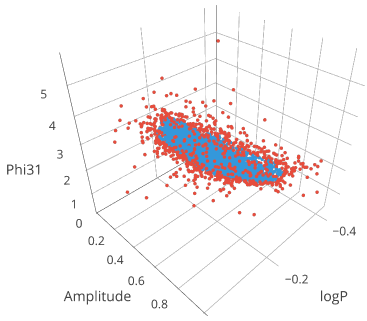
\includegraphics[width=0.3\paperwidth]{images/ksvm_rbfdot.png} & 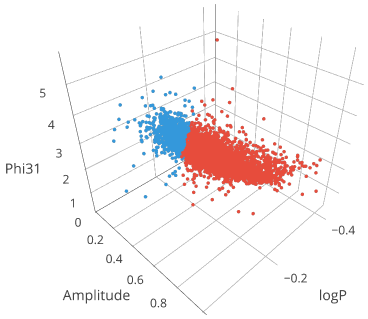
\includegraphics[width=0.3\paperwidth]{images/ksvm_polydot.png} \\
	\verb|rbfdot| & \verb|polydot| \\
	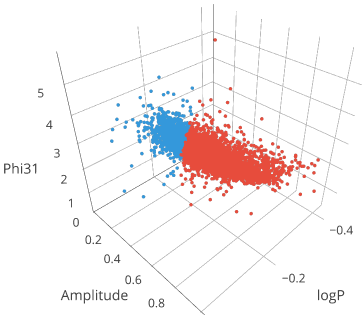
\includegraphics[width=0.3\paperwidth]{images/ksvm_vanilladot.png} & 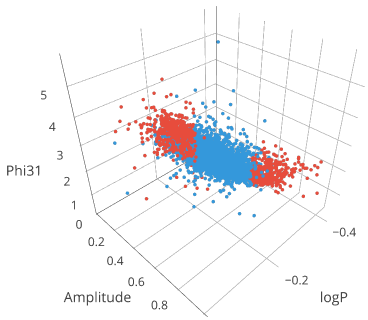
\includegraphics[width=0.3\paperwidth]{images/ksvm_tanhdot.png} \\
	\verb|vanilladot| & \verb|tanhdot| \\
	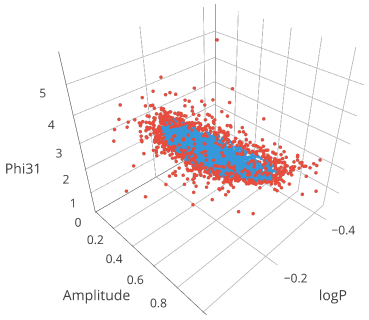
\includegraphics[width=0.3\paperwidth]{images/ksvm_laplacedot.png} & 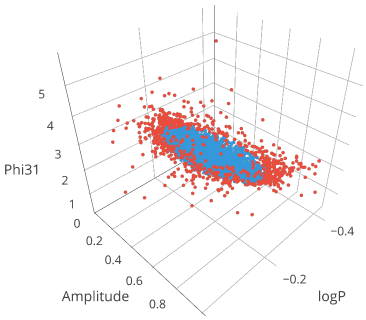
\includegraphics[width=0.3\paperwidth]{images/ksvm_besseldot.png} \\
	\verb|laplacedot| & \verb|besseldot| \\
	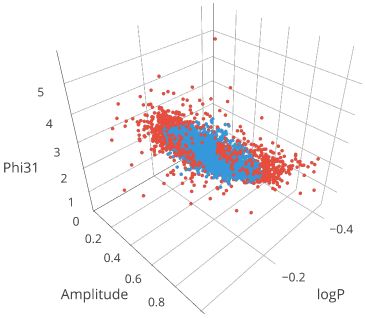
\includegraphics[width=0.3\paperwidth]{images/ksvm_anovadot.png} & 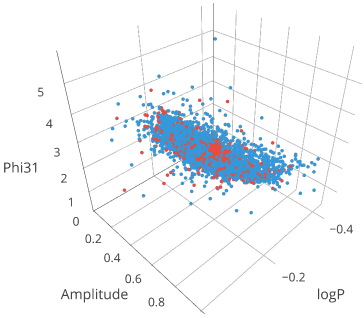
\includegraphics[width=0.3\paperwidth]{images/ksvm_splinedot.png} \\
	\verb|anovadot| & \verb|splinedot| \\
\end{longtable}

